\chapter{State of Art}
\section{Planowanie operacji antyterrorystycznych w~rzeczywistości}
Problem terroryzmu i skutków, jakie może on wyrządzać ludności, jest dla instytucji państwowych podstawą do przygotowywania długoterminowych strategii jego zapobiegania. Strategie te ujęte są w dokumentach\footnote{polskim przykładem jest dokument "Narodowy Program Antyterrorystyczny RP na lata 2012-2016"} przygotowywanych przez instrumenty państwowe. Opisują one środki i metody zabezpieczania obywateli przed aktami terroryzmu. Niestety, w zetknięciu z rzeczywistością bywają one nie zawsze skuteczne.

Mając do czynienia z aktem terroryzmu, polegającym na przejęciu kontroli przez terrorystów nad pewną przestrzenią (np. nad budynkiem), służby odpowiadające za bezpieczeństwo podejmują szereg działań, które mają na celu zminimalizować ryzyko utraty zdrowia lub życia przez osoby postronne (w tym ew. zakładników). Prócz zabezpieczenia okolicznego terenu (odizolowaniu go od cywili oraz mediów) oraz prowadzenia negocjacji z terrorystami, bardzo ważnym elementem jest przygotowanie planu przejęcia zakładników oraz ew. eliminacji terrorystów z użyciem siły. Do takiej czynności może dojść w przypadku, gdy terroryści odmówią negocjacji, bądź gdy zaczynają zabijać zakładników.

Proces planowania akcji antyterrorystycznych jest często charakterystyczny dla przeprowadzającej go jednostki specjalnej i zawsze jest strzeżony tajemnicą. Jednakże na przełomie kwietnia i maja 1980 roku, gdy grupa sześciu terrorystów przejęła kontrolę nad Ambasadą Irańską w Londynie, biorąc za zakładników 26 osób, to brytyjskie jednostki specjalne przeprowadziły skuteczną eliminację terrorystów na oczach całego świata\footnote{świadkami operacji byli dziennikarze wielu stacji telewizyjnych, a wśród zakładników byli m. in. reporterzy BBC}. Dzisiaj Operacja Nimrod jest szczegółowo udokumentowana licznymi artykułami\footnote{przy przygotowywaniu tej pracy został wykorzystany artykuł ze strony Elite UK Forces\cite{eliteUK}}, książkami oraz dokumentami wideo. Dzięki tej wiedzy jesteśmy w stanie odtworzyć proces planowania takiej akcji antyterrorystycznej, co zostało ukazane w tabeli \ref{realPlan}. Spełnienie wszystkich wymienionych czynności znacznie zwiększa szanse na powodzenie operacji: uratowanie zakładników, eliminacja terrorystów i nieodniesienie strat własnych przez jednostkę przeprowadzającą atak.

\begin{table}
\begin{center}
\begin{tabular}{p{0.5\textwidth} p{0.5\textwidth}}
Planowana czynność & Realizacja (Nimrod)\\\hline
	\begin{enumerate}
		\setlength\itemsep{0pt}
		\item Przygotowanie IA Plan\footnote{Immediate Action Plan - plan eliminacji terrorystów, który jest przygotowywany przed powstaniem docelowego planu (najczęściej w tym czasie nie ma jeszcze danych wywiadowczych)}
		\item Zbieranie danych
		\item Rozpoznanie wroga
		\item Rozpoznanie wyposażenia wroga
		\item Rozpoznanie terenu
		\item Określenie niezbędnych środków 
		\item Określenie punktów wejścia
		\item Określenie punktów ewakuacji		
	\end{enumerate}&\begin{enumerate}
		\setlength\itemsep{0pt}
		\item Szturm ambasady od głównego wejścia i zabezpieczanie budynku piętro po piętrze
		\item Zainstalowane podsłuchy w ścianach, snajperzy jako obserwatorzy, sprawdzanie punktów wejścia pod osłoną nocy
		\item Wywiad dostarcza dane osobowe terrorystów, którzy starali się o~wizy w ambasadzie Wielkiej Brytanii w Belgradzie
		\item Jeden z uwolnionych zakładników informuje policję o liczbie i uzbrojeniu terrorystów
		\item Analizowane są plany architektoniczne budynku i prowadzona jest konsultacja z woźnym ambasady
		\item Cztery drużyny (24 żołnierzy), pistolety maszynowe MP5, ładunki wybuchowe, granaty ogłuszające, liny itp.
		\item Wejście przez dach, wejście przez balkony na pierwszym piętrze, wejście tylnymi drzwiami na parterze
		\item Ewakuacja zakładników do ogrodu za budynkiem ambasady
	\end{enumerate}
\end{tabular}
\caption {Czynności dokonywane podczas planowania operacji antyterrorystycznej\label{realPlan}}
\end{center}
\end{table} 

W grze symulacyjnej, będącej przedmiotem tej pracy dyplomowej, gracz może zaplanować podstawowe elementy operacji antyterrorystycznej:
\begin{enumerate}
	\item zdefiniować liczbę terrorystów i antyterrorystów
	\item zaplanować jednopoziomową architekturę budynku
	\item oznaczyć punkty kluczowe wokół których można spodziewać się obecności terrorystów
	\item zdefiniować punkt wejścia oraz punkt ewakuacji
\end{enumerate}

\section{Gry symulacyjne}
Gatunek gier symulacyjnych charakteryzuje się wiernym odzwierciedlaniem realiów świata rzeczywistego lub fikcyjnego. Prócz zastosowania rozrywkowego, gry symulacyjne wykorzystuje się do celów szkoleniowych (np. wirtualna nauka jazdy) lub badawczych (np. analiza bezpieczeństwa terytorialnego). Wśród symulacyjnych gier wideo należy wymieć kilka podgatunków\footnote{przedstawiona lista wywodzi się z podziału przedstawionego w książce A. Rollingsa i E. Adamsa\cite{gameDesign} i dopełniona jest podgatunkami omawianymi w różnych publikacjach internetowych}:

\begin{description}
	\item[Symulatory budowania i zarządzania] cechują się brakiem obecności wroga, którego gracz musi pokonać. Są to gry o pewnych procesach (ekonomicznych, politycznych, wytwórczych itp.), w ramach których gracz odgrywa rolę architekta i zarządcy. Obiektami budowanymi mogą być parki rozrywki, porty lotnicze, szpitale, zoo czy też miasta. Im lepiej gracz rozumie zachodzące procesy, tym skuteczniejszy w wykonywaniu powierzonych mu zadań. Pierwszym symulatorem tego typu była gra \textbf{SimCity} [Maxis 1989].
	\item[Symulatory życia] pozwalają na kontrolowanie istnień i rozwijaniu relacji między nimi. Mechanizmy są to podobne do symulatorów budowania i zarządzania i często nie ma określonego kryterium zwycięstwa. Gry symulacyjne, gdzie gracz hoduje zwierzę lub jakiś antropomorficzny twór, skupiają się na tworzeniu i rozwijaniu relacji tej formy życia z graczem. Przykładami takich gier jest \textbf{The Sims} [Maxis 2000] oraz \textbf{Spore} [Maxis 2008].
	\item[Symulatory sportowe] pozwalają graczowi na wirtualne uprawianie dyscyplin sportowych, których zasady i kryteria zwycięstwa są zgodne z rzeczywistymi odpowiednikami\footnote{choć część zasad może być wyłączana, np. czas trwania meczu piłkarskiego lub błąd kroków w~koszykówce}. Często takie symulatory wymagają od swoich twórców modelowania rzeczywistych postaci ze świata sportu, wraz z uwzględnieniem ich umiejętności, charakterystycznych ruchów czy ubioru. Przykładami takich gier są gry z serii \textbf{Pro Evolution Soccer} [Konami] oraz \textbf{NBA Live} [EA Sports].
	\item[Symulatory pojazdów] mają na celu dostarczyć graczom wrażeń, jakie mogliby odczuć podczas kierowania rzeczywistymi pojazdami, w określonych warunkach. Tego typu gry najcześciej charakteryzują się bardzo wysoką wiernością odzwierciedlenia pojazdów, do której należy zaliczyć takie czynniki, jak wygląd, parametry jazdy lub lotu, wyposażenie oraz sterowanie. Przykładami takich gier jest seria \textbf{Colin McRae Rally} [Codemasters] oraz seria \textbf{Microsoft Flight Simulator} [Microsoft].
	\item[Symulatory czynności i zawodów] to dość popularny w ostatnim czasie typ gier. Mają one na celu umożliwienie graczom na wirtualne wykonywanie prac związanych z zawodami, którymi na co dzień się nie zajmują. Przykładami takich gier jest \textbf{Symulator Farmy 2011} [Atari / Infogrames 2011] czy \textbf{Symulator Koparki 2011} [astragon Software 2011]. Realizm nie jest tutaj najważniejszym kryterium.
\end{description}

Grę symulacyjną, będącą przedmiotem tej pracy dyplomowej, można sklasyfikować w podgatunku symulatorów czynności i zawodów.

\section{Sztuczna inteligencja w grach}
Sztuczna inteligencja, jako dział informatyki, zajmuje się analizą zachowań człowieka oraz formalizowaniem (np. w postaci algorytmów) zaobserwowanych procesów m.in. myślowych i decyzyjnych. Dzięki takiej analizie jest możliwe przygotowywanie programów, pozwalających na rozwiązywanie problemów, które do tej pory były domeną ludzką. Przykładami mogą tu być wyszukiwanie danych, rozpoznawanie obiektów, syntezacja mowy lub podejmowanie decyzji. W tym celu algorytmy sztucznej inteligencji mogą wykorzystywać implementacje takich zagadnień, jak sieci neuronowe, algorytmy genetyczne czy logika rozmyta.

W grach wideo sztuczna inteligencja najczęściej sprowadza się do zastosowania prostych technik sztucznej inteligencji, które mają na celu zaspokoić trzy podstawowe potrzeby bohaterów gry\cite{aiForGames}:
\begin{itemize}
	\item zdolność poruszania się 
	\item zdolność do podejmowania decyzji gdzie należy się poruszyć
	\item zdolność taktycznego i strategicznego myślenia
\end{itemize}

\begin{figure}
\begin{center}
	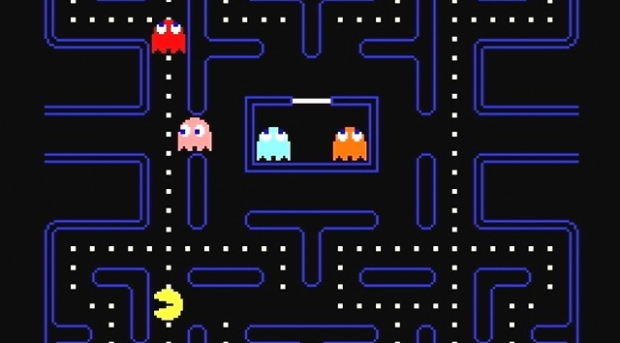
\includegraphics[width=120mm,height=66mm]{images/pacman}
	\caption{Pac-Man - przykład prostych technik sztucznej inteligencji w grach\label{pacman}}
\end{center}
\end{figure}

\textbf{Pac-Man} [Namco, 1980] była jedną z pierwszych gier, która posiadała zauważalne dla odbiorców elementy sztucznej inteligencji. Gracz, poruszając się po dwuwymiarowym labiryncie, zdobywał punkty zjadając kropki (rysunek \ref{pacman}). W tej czynności aktywnie przeszkadzały mu cztery duchy, które starały się podążać korytarzami labiryntu w kierunku gracza. Od strony implementacyjnej gra opierała się o bardzo prostą maszynę stanową, która dla duchów definiowała dwa stany: podążaj za graczem i uciekaj od gracza. Na każdym skrzyżowaniu dróg labiryntu podejmowana była decyzja\footnote{decyzja była losowa lub poparta prostymi obliczeniami} o następnym kierunku.

W późniejszych grach elementy myślenia i podejmowania decyzji stawały się coraz bardziej rozbudowane. Przykładem jest gra \textbf{Goldeneye 007} [Rare Ltd. 1997], gdzie postaci zostały wyposażone w system symulowanych zmysłów. Jedna postać analizowała pulę informacji ze świata gry, co pozwalało np. na dostrzeżenie martwego towarzysza i wykonanie odpowiedniej reakcji na ten fakt - czyli zmiany własnego stanu.

\begin{figure}
\begin{center}
	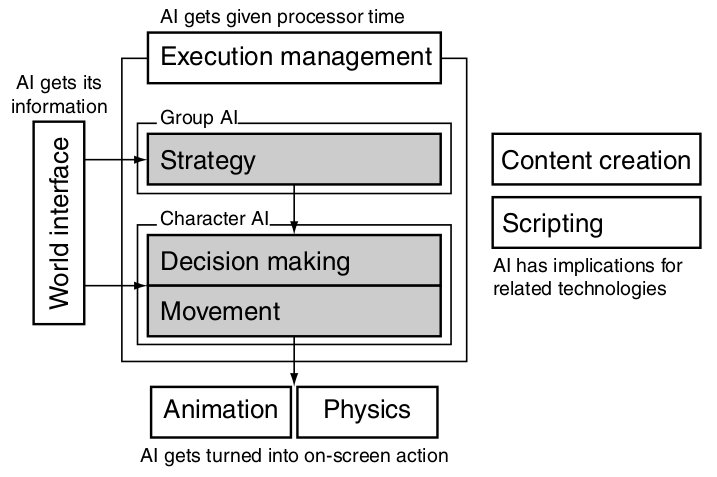
\includegraphics[width=120mm,height=80mm]{images/aimodel}
	\caption{AI Model - zdefiniowany przez I. Millingtona i J. Funge\label{aimodel}}
\end{center}
\end{figure}

Analizując elementy składowe sztucznej inteligencji w grach wideo, należy odwołać się do modelu AI (rysunek \ref{aimodel}). Postaci z gry posiadają wiedzę (całościową lub cząstkową) o świecie w którym funkcjonują (\emph{World interface}). Na podstawie tej wiedzy każda postać, za pomocą odpowiednich algorytmów, podejmuje jakieś decyzje (\emph{Decision making}) oraz porusza się (\emph{Movement}). Element strategii (\emph{Strategy}) jest przetwarzany na poziomie grupy postaci i może wpływać na podejmowane przez jednostki decyzje lub wykonywane ruchy. Rezultatem bezpośrednim tych obliczeń są wykonywane animacje (\emph{Animation}) oraz wyliczenia fizyki ruchu postaci (\emph{Physics}). Efektem ubocznym mogą tu być zmiany stanu gry, polegające na modyfikacji elementów świata (\emph{Content creation}) gry oraz wykonywaniu oskryptowanych akcji (\emph{Scripting}).

W grze symulacyjnej, będącą przedmiotem tej pracy dyplomowej, będziemy mogli wyróżnić każdy z trzech elementów modelu sztucznej inteligencji:
\begin{description}
	\item[Podejmowanie decyzji] np. otwarcie ognia do wroga lub ucieczka
	\item[Poruszanie się] np. poruszanie po ścieżce, wędrowanie
	\item[Strategia] np. role i ich przejmowanie w grupie antyterrorystów
\end{description}

\section{Istniejące rozwiązania: gra Rainbox Six}


\section{HTML5 Canvas i Javascript}

